% ------------------------------------------------------------------------------
% TYPO3 CMS 8 LTS - What's New - Chapter "In-Depth Changes" (Dutch Version)
%
% @author	Michael Schams <schams.net>
% @license	Creative Commons BY-NC-SA 3.0
% @link		http://typo3.org/download/release-notes/whats-new/
% @language	English
% ------------------------------------------------------------------------------
% LTXE-CHAPTER-UID:		5ebcecbe-66abfa57-cf38bc00-aa637965
% LTXE-CHAPTER-NAME:	In-Depth Changes
% ------------------------------------------------------------------------------

\section{Systeemwijzigingen}
\begin{frame}[fragile]
	\frametitle{Systeemwijzigingen}

	\begin{center}\huge{\color{typo3darkgrey}\textbf{Systeemwijzigingen}}\end{center}
	\begin{center}\large{\textit{Geweldige nieuwe functies en verbeteringen binnenin}}\end{center}

\end{frame}

% ------------------------------------------------------------------------------
% LTXE-SLIDE-START
% LTXE-SLIDE-UID:		e977cd44-05efc4d0-66d25874-3e8ec5f2
% LTXE-SLIDE-ORIGIN:	b9b259e4-9d35ace7-edff1014-7390d1d1 English
% LTXE-SLIDE-TITLE:		#69794: Support PECL-memcached in MemcachedBackend
% ------------------------------------------------------------------------------
\begin{frame}[fragile]
	\frametitle{Systeemwijzigingen}
	\framesubtitle{Ondersteuning PECL-memcached in MemcachedBackend}

	% decrease font size for code listing
	\lstset{basicstyle=\tiny\ttfamily}

	\begin{itemize}

		\item Ondersteuning voor de PECL-module "memcached" is toegevoegd aan de
			MemcachedBackend van het Caching Framework

		\item Als zowel "memcache" als "memcached" zijn geïnstalleerd, wordt "memcache"
			gebruikt om geen brekende wijziging te zijn.

		\item Een integrator kan de optie \texttt{peclModule} gebruiken om de voorkeur
			in te stellen:

			\begin{lstlisting}
				$GLOBALS['TYPO3_CONF_VARS']['SYS']['caching']['cacheConfigurations']['my_memcached'] = [
				  'frontend' => \TYPO3\CMS\Core\Cache\Frontend\VariableFrontend::class
				  'backend' => \TYPO3\CMS\Core\Cache\Backend\MemcachedBackend::class,
				  'options' => [
				    'peclModule' => 'memcached',
				    'servers' => [
				      'localhost',
				      'server2:port'
				    ]
				  ]
				];
			\end{lstlisting}

	\end{itemize}

\end{frame}


% ------------------------------------------------------------------------------
% LTXE-SLIDE-START
% LTXE-SLIDE-UID:		b33bcdfc-f1e7922b-c07ac715-b08f412d
% LTXE-SLIDE-ORIGIN:	ef8c124e-f902453a-d48770b9-4cf86545 English
% LTXE-SLIDE-TITLE:		#73042: Native support for Symfony Console (1)
% ------------------------------------------------------------------------------
\begin{frame}[fragile]
	\frametitle{Systeemwijzigingen}
	\framesubtitle{Ondersteuning voor Symfony Console (1)}

	% decrease font size for code listing
	\lstset{basicstyle=\tiny\ttfamily}

	\begin{itemize}

		\item TYPO3 ondersteunt de Symfony Console automatisch via een nieuw commandoregel
			script in \texttt{typo3/sysext/core/bin/typo3}.
			Bij TYPO3-installaties die via Composer zijn gemaakt wordt het uitvoerbare bestand
			gekoppeld aan de \texttt{bin}-folder, bijv. \texttt{bin/typo3}.

		\item Het nieuwe script ondersteunt nog steeds de bestaande argumenten als er geen
			correct Symfony Console-commando wordt gevonden.

		\item Een commando dat via de TYPO3-commandoregel beschikbaar moet zijn, kan
		 	geregistreerd worden door het plaatsen van een \texttt{Configuration/Commands.php}-bestand
		 	in een geïnstalleerde extensie. De lijst Symfony/Console/Command klassen die uitgevoerd
		 	kunnen worden door TYPO3, is een hash-tabel. De index is de naam van het commando
		 	dat als eerste argument voor TYPO3 gebruikt wordt.

	\end{itemize}

\end{frame}

% ------------------------------------------------------------------------------
% LTXE-SLIDE-START
% LTXE-SLIDE-UID:		8f20da1f-c56db343-fc77a12a-283aa580
% LTXE-SLIDE-ORIGIN:	28b018bb-21804fa1-c578f0ff-fc16cbb1 English
% LTXE-SLIDE-TITLE:		#73042: Native support for Symfony Console (2)
% ------------------------------------------------------------------------------
\begin{frame}[fragile]
	\frametitle{Systeemwijzigingen}
	\framesubtitle{Ondersteuning voor Symfony Console (2)}

	% decrease font size for code listing
	\lstset{basicstyle=\tiny\ttfamily}

	\begin{itemize}

		\item Een vereiste parameter bij het registreren van een commando is de \texttt{class}-eigenschap.
			Optioneel kan de \texttt{user}-parameter ingesteld worden zodat een backend gebruiker ingelogd
			is bij het aanroepen van het commando.

		\item Een \texttt{Configuration/Commands.php} kan er zo uitzien:

			\begin{lstlisting}
				return [
				  'backend:lock' => [
				    'class' => \TYPO3\CMS\Backend\Command\LockBackendCommand::class
				  ],
				  'referenceindex:update' => [
				    'class' => \TYPO3\CMS\Backend\Command\ReferenceIndexUpdateCommand::class,
				    'user' => '_cli_lowlevel'
				  ]
				];
			\end{lstlisting}

	\end{itemize}

\end{frame}

% ------------------------------------------------------------------------------
% LTXE-SLIDE-START
% LTXE-SLIDE-UID:		a3da7fbb-338025fb-6072a65d-7964e8e5
% LTXE-SLIDE-ORIGIN:	fc16cbb1-21804fa1-c578f0ff-28b018bb English
% LTXE-SLIDE-TITLE:		#73042: Native support for Symfony Console (3)
% ------------------------------------------------------------------------------
\begin{frame}[fragile]
	\frametitle{Systeemwijzigingen}
	\framesubtitle{Ondersteuning voor Symfony Console (3)}

	% decrease font size for code listing
	\lstset{basicstyle=\tiny\ttfamily}

	\begin{itemize}

		\item Een aanroep kan er zo uitzien:
			\begin{lstlisting}
				bin/typo3 backend:lock http://example.com/maintenance.html
			\end{lstlisting}

		\item Voor een niet-Composer-installatie:
			\begin{lstlisting}
				typo3/sysext/core/bin/typo3 backend:lock http://example.com/maintenance.html
			\end{lstlisting}

	\end{itemize}

\end{frame}


% ------------------------------------------------------------------------------
% LTXE-SLIDE-START
% LTXE-SLIDE-UID:		2078dd2b-51381b9a-d3a2a084-007eb0c5
% LTXE-SLIDE-ORIGIN:	dd31e5d5-ca09ae5e-eb87d926-0ffe8f0a English
% LTXE-SLIDE-TITLE:		Low-level parameters changes (1)
% ------------------------------------------------------------------------------
\begin{frame}[fragile]
	\frametitle{Systeemwijzigingen}
	\framesubtitle{Parameterwijzigingen in Low-level (1)}

	% changes: #78417, #78439, #78520, #78552, #78577, #78623, #78627 and #78895

	\begin{itemize}
		\item Low-level commando's in de lijst hieronder gebruiken nu de Symfony Console
		\item Nieuwe commando's werken zoals de oude, maar ondersteunen bepaalde parameters

			\begin{itemize}
				\item \texttt{DeletedRecordsCommand}
				\item \texttt{CleanFlexFormsRecordsCommand}
				\item \texttt{OrphanRecordsCommand}
				\item \texttt{LostFilesCommand}
				\item \texttt{MissingFilesCommand}
				\item \texttt{MissingRelationsCommand}
				\item \texttt{DoubleFilesCommand}
				\item \texttt{RteImagesCommand}
			\end{itemize}

	\end{itemize}

\end{frame}

% ------------------------------------------------------------------------------
% LTXE-SLIDE-START
% LTXE-SLIDE-UID:		ae77fc7a-1e3be981-7fc306a5-f05ea0b3
% LTXE-SLIDE-ORIGIN:	3a9d25bb-d948368d-e2a92666-6170eaad English
% LTXE-SLIDE-TITLE:		Low-level parameters changes (2)
% ------------------------------------------------------------------------------
\begin{frame}[fragile]
	\frametitle{Systeemwijzigingen}
	\framesubtitle{Parameterwijzigingen in Low-level (2)}

	% changes: #78417, #78439, #78520, #78552, #78577, #78623, #78627 and #78895

	\begin{itemize}
		\item Gerelateerde PHP klassen zijn verwijderd\newline
			\smaller(e.g. \texttt{TYPO3\textbackslash
				CMS\textbackslash
				Lowlevel\textbackslash
				DeletedRecordsCommand})
			\normalsize

		\item Het commando via \texttt{cli\_dispatch} werkt niet meer\newline
			\smaller(bijv. \texttt{typo3/cli\_dispatch lowlevel cleaner deleted})\normalsize
		\item Aanroepen van de PHP klasse geeft nu een PHP-fout

		\item Commando's kunnen nu uitgevoerd worden via CLI als volgt:\newline
			\smaller\texttt{/typo3/sysext/core/bin/typo3 cleanup:<command>}\normalsize\newline
			bijvoorbeeld:\newline
			\smaller\texttt{/typo3/sysext/core/bin/typo3 cleanup:deletedrecords}\normalsize

	\end{itemize}

\end{frame}

% ------------------------------------------------------------------------------
% LTXE-SLIDE-START
% LTXE-SLIDE-UID:		a31ed742-5c4952f6-05a4f158-1e0c5441
% LTXE-SLIDE-ORIGIN:	1626edc6-8d93ff84-f64178bf-8e7650df English
% LTXE-SLIDE-TITLE:		#73050: Cryptographically secure pseudorandom number generator
% ------------------------------------------------------------------------------
\begin{frame}[fragile]
	\frametitle{Systeemwijzigingen}
	\framesubtitle{Cryptografisch veilige pseudotoevalsgenerator}

	% decrease font size for code listing
	\lstset{basicstyle=\tiny\ttfamily}

	\begin{itemize}

		\item Een nieuwe cryptografisch veilige pseudotoevalsgenerator (CSPRNG) is
			geïmplementeerd in de TYPO3 core.\newline
			Het gebruikt de nieuwe CSPRNG-functies in PHP 7.

		\item De API zit in de klasse
			\texttt{\textbackslash
				TYPO3\textbackslash
				CMS\textbackslash
				Core\textbackslash
				Crypto\textbackslash
				Random}

		\item Voorbeeld:

			\begin{lstlisting}
				use \TYPO3\CMS\Core\Crypto\Random;
				use \TYPO3\CMS\Core\Utility\GeneralUtility;

				// Willekeurige bytes ophalen
				$someRandomString = GeneralUtility::makeInstance(Random::class)->generateRandomBytes(64);

				// Dobbelsteen rollen...
				$tossedValue = GeneralUtility::makeInstance(Random::class)->generateRandomInteger(1, 6);
			\end{lstlisting}

	\end{itemize}

\end{frame}

% ------------------------------------------------------------------------------
% LTXE-SLIDE-START
% LTXE-SLIDE-UID:		a7689389-3ecab162-50dbfeed-5f923019
% LTXE-SLIDE-ORIGIN:	2c656d9e-38b9be7a-d590cb6e-21eccd4d English
% LTXE-SLIDE-TITLE:		#28230: Password hashing algorithm: PBKDF2
% ------------------------------------------------------------------------------
\begin{frame}[fragile]
	\frametitle{Systeemwijzigingen}
	\framesubtitle{Algoritme voor wachtwoordhash: PBKDF2}

	\begin{itemize}

		\item Een nieuw hash-algoritme voor wachwoorden, "PBKDF2", is toegevoegd aan de systeemextensie "saltedpasswords"

		\item PBKDF2 betekent: Password-Based Key Derivation Function 2

		\item Het algoritme kost veel rekenkracht om brute force password cracking te weerstaan

	\end{itemize}

\end{frame}

% ------------------------------------------------------------------------------
% LTXE-SLIDE-START
% LTXE-SLIDE-UID:		40f1577d-905a4f91-dcf7e814-84789fd9
% LTXE-SLIDE-ORIGIN:	630de169-c2699a8a-ee44dde5-cf39c2ca English
% LTXE-SLIDE-TITLE:		#70056 - PHP Library "Guzzle" (1)
% ------------------------------------------------------------------------------
\begin{frame}[fragile]
	\frametitle{Systeemwijzigingen}
	\framesubtitle{PHP Bibliotheek "Guzzle" (1)}

	\begin{itemize}

		\item De PHP-bibliotheek
			"\href{http://docs.guzzlephp.org}{Guzzle}"
			is toegevoegd via een composerafhankelijkheid als oplossing voor het
			maken van HTTP aanvragen gebaseerd op de PSR-7 interfaces die al
			door TYPO3 gebruikt worden

		\item Guzzle detecteert vanzelf welke onderliggende adapters -- zoals
		 	cURL or stream wrappers -- beschikbaar zijn en kiest dan de beste
		 	oplossing voor het systeem

		\item Een TYPO3-specifiek PHP-klasse
			\texttt{TYPO3\textbackslash
				CMS\textbackslash
				Core\textbackslash
				Http\textbackslash
				RequestFactory}\newline
			is toegevoegd als simpele wrapper voor toegang tot Guzzle clienten

	\end{itemize}

\end{frame}


% ------------------------------------------------------------------------------
% LTXE-SLIDE-START
% LTXE-SLIDE-UID:		0c1dd60b-f7366c17-c86200bf-b67b25a0
% LTXE-SLIDE-ORIGIN:	db2b31c1-47321ffe-3ed51ebc-5dd524a4 English
% LTXE-SLIDE-TITLE:		#70056 - PHP Library "Guzzle" (2)
% ------------------------------------------------------------------------------
\begin{frame}[fragile]
	\frametitle{Systeemwijzigingen}
	\framesubtitle{PHP Bibliotheek "Guzzle" (2)}

	% decrease font size for code listing
	\lstset{basicstyle=\tiny\ttfamily}

	\begin{itemize}

		\item De \texttt{RequestFactory} klasse kan zo gebruikt worden:

			\begin{lstlisting}
				// Initialiseer RequestFactory

				/** @var \TYPO3\CMS\Core\Http\RequestFactory $requestFactory */
				$requestFactory = GeneralUtility::makeInstance(
				  \TYPO3\CMS\Core\Http\RequestFactory\RequestFactory::class);

				$uri = $additionalOptions = [
				  // extra headers voor deze opdracht
				  'headers' => ['Cache-Control' => 'no-cache'],
				  'allow_redirects' => false,
				  'cookies' => true
				];

				// geef een PSR-7 response object terug
				$response = $requestFactory->request($url, 'GET', $additionalOptions);

				// haal de inhoud op als string bij een succesvolle opdracht
				if ($response->getStatusCode() === 200) {
				  if ($response->getHeader('Content-Type') === 'text/html') {
				    $content = $response->getBody()->getContents();
				  }
				}
			\end{lstlisting}

	\end{itemize}

\end{frame}

% ------------------------------------------------------------------------------
% LTXE-SLIDE-START
% LTXE-SLIDE-UID:		a5bfc71f-f1abfaf3-77635f52-423f728f
% LTXE-SLIDE-ORIGIN:	bd33b29d-c20d1765-f923f78e-43bfb0bf English
% LTXE-SLIDE-TITLE:		#74365: Add Linkservice for Unified Referencing Syntax (1)
% ------------------------------------------------------------------------------
\begin{frame}[fragile]
	\frametitle{Systeemwijzigingen}
	\framesubtitle{Linkservice voor standaard verwijzingssyntax (1)}

	\begin{itemize}

		\item Binnen TYPO3 werd er op verschillende manieren verwezen naar bronnnen.

		\item TYPO3 ondersteunt nu een moderne, toekomstzekere manier om naar bronnen te verwijzen met een uitbreidbare en
			duidelijk syntax die eenvoudig te begrijpen is.

		\item De volgende pagina's leggen de syntax uit met de volgende, simpele link naar een pagina:

			\begin{lstlisting}
				t3://page?uid=13&campaignCode=ABC123
			\end{lstlisting}

	\end{itemize}

\end{frame}

% ------------------------------------------------------------------------------
% LTXE-SLIDE-START
% LTXE-SLIDE-UID:		830d8a0f-bc469ca7-f7113776-41373c15
% LTXE-SLIDE-ORIGIN:	95f9a663-ea2155a1-5635728b-77a8995c English
% LTXE-SLIDE-TITLE:		#74365: Add Linkservice for Unified Referencing Syntax (2)
% ------------------------------------------------------------------------------
\begin{frame}[fragile]
	\frametitle{Systeemwijzigingen}
	\framesubtitle{Linkservice voor standaard verwijzingssyntax (2)}

	\begin{itemize}

		\item De syntax bestaat uit drie delen:

			\begin{itemize}

				\item Namespace (\texttt{t3://})\newline
		   			De namespace is altijd \texttt{t3://} om te zorgen dat de "LinkService" wordt uitgevoerd voor deze URN.
					\newline
				\item Sleutel van bronbehandelaar (\texttt{page})\newline
   					De sleutel van de bronbehandelaar is een lijst van behandelaars die beschikbaar zijn in TYPO3.
   					Momenteel bestaan de volgende behandelaars: \texttt{page}, \texttt{file} en \texttt{folder}.\newline
					Meer sleutels kunnen geconfigureerd worden in een associatieve array waarbij de index de behandelaarsleutel is
					en de waarde een klasse is die de LinkHandlerInterface implementeert:\newline
					\texttt{\$TYPO3\_CONF\_VARS['SYS']['linkHandler']}

			\end{itemize}

	\end{itemize}

\end{frame}

% ------------------------------------------------------------------------------
% LTXE-SLIDE-START
% LTXE-SLIDE-UID:		e2dc55c4-8681609d-fbd79573-83664fac
% LTXE-SLIDE-ORIGIN:	77a8995c-ea2155a1-95f9a663-5635728b English
% LTXE-SLIDE-TITLE:		#74365: Add Linkservice for Unified Referencing Syntax (3)
% ------------------------------------------------------------------------------
\begin{frame}[fragile]
	\frametitle{Systeemwijzigingen}
	\framesubtitle{Linkservice voor standaard verwijzingssyntax (3)}

	\begin{itemize}

		\item ...en deel 3:

			\begin{itemize}

				\item Bronparameters (\texttt{?uid=13\&campaignCode=ABC123})\newline
					Dit zijn de specifieke identificatieparameters die gebruikt worden door een behandelaar.
					Let op dat deze extra parameters kunnen bevatten om het gedrag van een behandelaar te bepalen.

			\end{itemize}

	\end{itemize}

\end{frame}

% ------------------------------------------------------------------------------
% LTXE-SLIDE-START
% LTXE-SLIDE-UID:		465f77fb-782f960f-2bc17884-e1d87199
% LTXE-SLIDE-ORIGIN:	af8e73a4-2b315873-bb6e55e4-c0cd82b5 English
% LTXE-SLIDE-TITLE:		#76008 and #76458: DebuggerUtility::var_dump (1)
% ------------------------------------------------------------------------------
\begin{frame}[fragile]
	\frametitle{Systeemwijzigingen}
	\framesubtitle{\texttt{DebuggerUtility::var\_dump} (1)}

	\begin{itemize}

		\item Informatie over de zichtbaarheid van een eigenschap is toegevoegd aan \texttt{DebuggerUtility::var\_dump()}
			\newline
			voor elke eigenschap van een object in de uitvoer

		\item Als een closure onderdeel is van het object dat gedebugd wordt, dan wordt de broncode hiervan ook afgebeeld

	\end{itemize}

	\tabto{0.75cm}\textit{Zie voorbeeld op de volgende pagina}

\end{frame}

% ------------------------------------------------------------------------------
% LTXE-SLIDE-START
% LTXE-SLIDE-UID:		c96bde6f-dae0cb08-25bd0caa-fdce062e
% LTXE-SLIDE-ORIGIN:	bb6e55e4-2b315873-c0cd82b5-af8e73a4 English
% LTXE-SLIDE-TITLE:		#76008 and #76458: DebuggerUtility::var_dump (2)
% ------------------------------------------------------------------------------
\begin{frame}[fragile]
	\frametitle{Systeemwijzigingen}
	\framesubtitle{\texttt{DebuggerUtility::var\_dump} (2)}

	\begin{figure}
		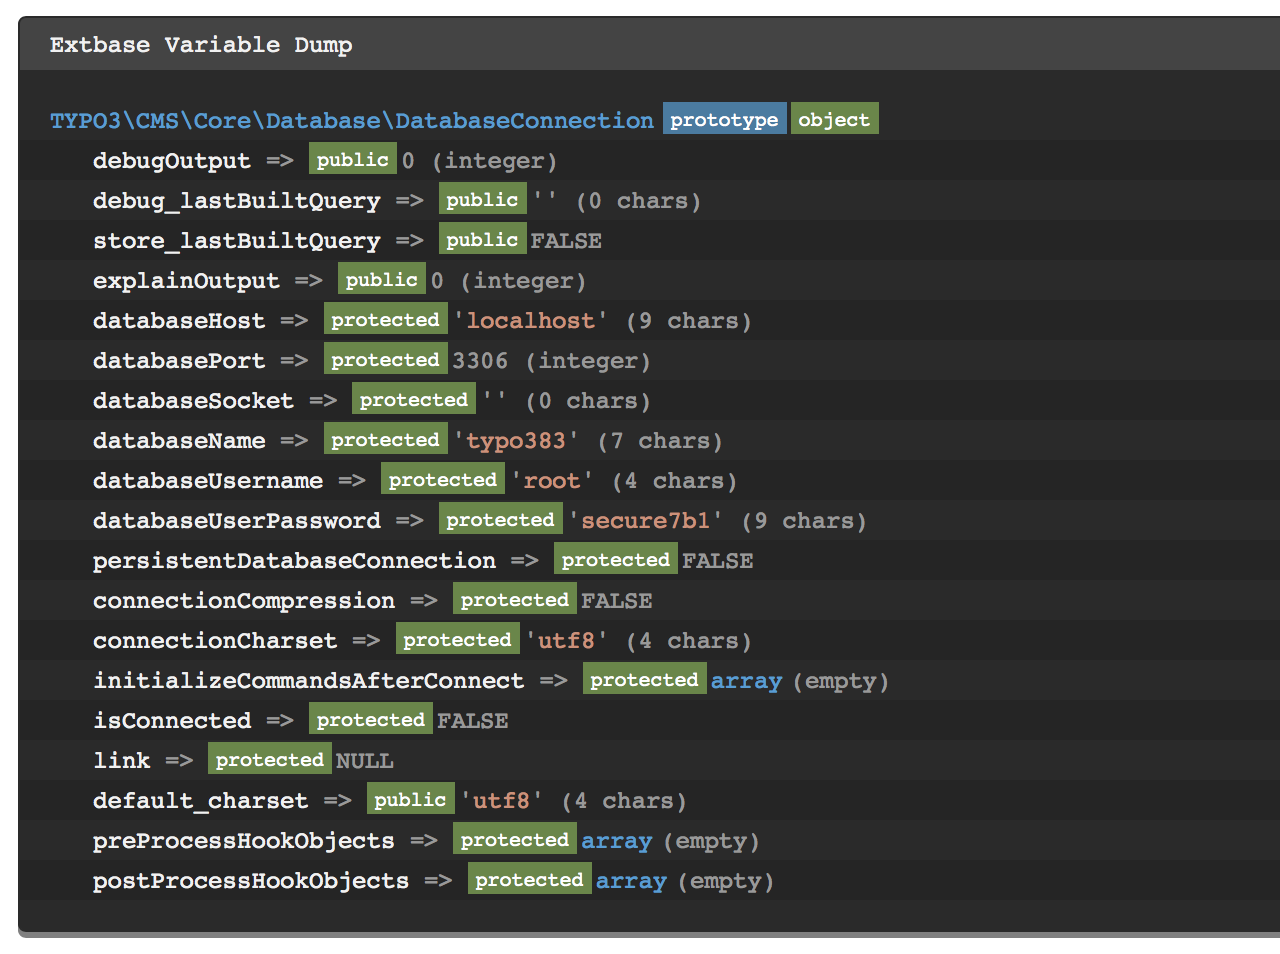
\includegraphics[width=0.65\linewidth]{InDepthChanges/76008.png}
	\end{figure}

\end{frame}

% ------------------------------------------------------------------------------
% LTXE-SLIDE-START
% LTXE-SLIDE-UID:		b359910a-13b7e044-d21d5eb5-ea249a5a
% LTXE-SLIDE-ORIGIN:	60a2d39f-f04b8bf1-dc758912-607ed07e English
% LTXE-SLIDE-TITLE:		#52286: System Status Updates Report via email
% ------------------------------------------------------------------------------
\begin{frame}[fragile]
	\frametitle{Systeemwijzigingen}
	\framesubtitle{Systeemstatus updates (rapportages)}

	\begin{itemize}
		\item Resultaten van tests in "Systeemstatus Updates (rapportages)" kunnen doorgemaild worden
		\item Een keuzevakje is toegevoegd aan de taakconfiguratie om:

			\begin{itemize}
				\item een e-mail te sturen als er waarschuwingen of foutmeldingen zijn
				\item altijd een e-mail te maken
			\end{itemize}

		\item Standaard worden alleen waarschuwingen en fouten opgenomen

	\end{itemize}

\end{frame}

% ------------------------------------------------------------------------------
% LTXE-SLIDE-START
% LTXE-SLIDE-UID:		d6e8762c-f8f590f0-3bfa3b98-0b956369
% LTXE-SLIDE-ORIGIN:	e4e2ead3-c07beb21-e8100580-d0e7c756 English
% LTXE-SLIDE-TITLE:		#58637: Purge language packs in language module
% ------------------------------------------------------------------------------

%\begin{frame}[fragile]
%	\frametitle{Systeemwijzigingen}
%	\framesubtitle{Language Packs}
%
%	\begin{itemize}
%		\item Deactivating languages in the module "Languages" left language data remaining
%			in directory \texttt{typo3conf/l10n/<locale>/}
%		\item A "remove"-button has been added, which disables the language and purges the
%			data in the directory
%	\end{itemize}
%
%\end{frame}

% ------------------------------------------------------------------------------
% LTXE-SLIDE-START
% LTXE-SLIDE-UID:		370dd7e3-508cef11-eeaf9991-250e09a4
% LTXE-SLIDE-ORIGIN:	73d888ce-a14c0f6a-d4dec5fb-f7368bb6 English
% LTXE-SLIDE-TITLE:		#76108, #77349 and #77481 Miscellaneous (1)
% ------------------------------------------------------------------------------
\begin{frame}[fragile]
	\frametitle{Systeemwijzigingen}
	\framesubtitle{Diversen (1)}

	\begin{itemize}

		\item SVGs en D3 rendering

			\begin{itemize}
				\item Als onderdeel van het verwijderen van ExtJS is de boom voor de formulieren opnieuw gebouwd
				\item Het renderen is gebaseerd op SVG's en D3 waardoor prestaties significant verbeteren
				\item Het opnieuw bouwen van de paginaboom op deze wijze is gepland voor de nabije toekomst
			\end{itemize}

		\item Iconen voor extensies kunnen opgeslagen worden in de directory:\newline
			\small
				\texttt{Resources/Public/Icons/<bestandsnaam>}
				(<bestandsnaam> kan zijn: \texttt{Extension.png}, \texttt{Extension.svg} or \texttt{Extension.gif})
			\normalsize

		\item De nieuwe opties \texttt{backendFavicon} in de configuratie van Extensiebeheer maakt het mogelijk om het favicon
			van de backend te wijzigen.

	\end{itemize}

\end{frame}

% ------------------------------------------------------------------------------
% LTXE-SLIDE-START
% LTXE-SLIDE-UID:		0a37dc0c-3165aea9-49e2c19b-25d39988
% LTXE-SLIDE-ORIGIN:	0907e5d3-a12751cb-23f49488-7a05a208 English
% LTXE-SLIDE-TITLE:		#78103, #78575 and #75232: Miscellaneous (2)
% ------------------------------------------------------------------------------
\begin{frame}[fragile]
	\frametitle{Systeemwijzigingen}
	\framesubtitle{Diversen (2)}

	% #78103: Add missing information status for addSystemMessage
	% #78575: Get enumeration constants
	% #75232: Spread TypeConverter priorities

	\begin{itemize}
		\item Alle systeeminformatie toegevoegd door \texttt{addSystemInformation()} heeft nu
			\texttt{InformationStatus::STATUS\_NOTICE} als standaard waarde
		\item De opsommingsconstanten kunnen nu eenvoudig opgehaald worden:

			\begin{itemize}
				\item \texttt{EnumerationClass::getName(\$value);}
				\item \texttt{EnumerationClass::getHumanReadableName(\$value);}
			\end{itemize}

		\item Prioriteiten van de TypeConverters uit de core zijn gewijzigd van \newline
			\texttt{1}, \texttt{2}, \texttt{3},... in \texttt{10}, \texttt{20}, \texttt{30},...
			Let bij het registreren van maatwerk TypeConverters op de juiste prioriteiten.

		\item \href{https://en.wikipedia.org/wiki/ISO_8601}{ISO-8601} wordt nu gebruikt om date en datetime
			waardes door te geven tussen server en de client. Eventueel moeten maatwerk FormEngine rendertypes
			bijgewerkt worden (\texttt{eval=date/datetime}).

	\end{itemize}

\end{frame}

% ------------------------------------------------------------------------------
